\documentclass[11pt]{article}
\usepackage[a4paper,margin=24mm]{geometry}
\usepackage{amsmath,amssymb,graphicx,booktabs,tabularx,array,url}
\usepackage[hidelinks]{hyperref}\usepackage{fontspec}
\setmainfont{Times New Roman}\setsansfont{Arial}\setmonofont{Menlo}
\usepackage{microtype}\setlength{\emergencystretch}{2em}
\newcommand{\Range}{\operatorname{Range}}
\renewcommand{\thefigure}{S\arabic{figure}}
\renewcommand{\thetable}{S\arabic{table}}
\title{Supplement: Maxwell Conditional Current Exchange\\Model, Locked Protocol, and Complete Evidence}
\author{}\date{}
% Use cached readable math sizes; no network font installation.
\DeclareMathSizes{10}{10}{7}{6}
\DeclareMathSizes{9}{9}{6}{6}
\DeclareMathSizes{8}{8}{6}{6}
\DeclareMathSizes{7}{7}{6}{6}
\DeclareMathSizes{6}{6}{6}{6}
\DeclareMathSizes{5}{6}{6}{6}
\begin{document}\maketitle
This supplement specifies the physical operators, numerical acceptance, validation population, and costs behind the receiver-centered exchange manuscript. Historical material-repair and solver controls are summarized separately; their original records remain unchanged in the accompanying archive. Current ranks refer to shared complex current columns, while material dimensions are real. Local full-GN fidelity and final material estimation are evaluated separately.
\setcounter{tocdepth}{1}\tableofcontents
\section{Physical model and shared material coordinates}
\subsection*{The continuous scattering picture}
The starting point is the vector-Maxwell volume-integral equation for an isotropic, nonmagnetic dielectric. For one illumination, write the induced current, or equivalently a consistently scaled contrast source, schematically as
\[
j(\boldsymbol r)=X(\boldsymbol r)\left[E^{\rm inc}(\boldsymbol r)
+\int_D G_D(\boldsymbol r,\boldsymbol r')j(\boldsymbol r')\,d\boldsymbol r'\right].
\]
Here $G_D$ maps source currents to the internal electric field, $X$ is the local material response, and the bracket is the total field $E^{\rm tot}$. The singular self-interaction is understood in the chosen Maxwell volume-integral convention; the implemented cell self-response is specified below. The physical constants associated with the source convention are included consistently in $X$ and the Green maps.

A small admissible change $\delta\chi$ changes both the local material response and the field produced by the currents. Differentiating at the current material state gives
\[
\delta j(\boldsymbol r)=DX[\delta\chi](\boldsymbol r)E^{\rm tot}(\boldsymbol r)
+X(\boldsymbol r)\int_DG_D(\boldsymbol r,\boldsymbol r')\delta j(\boldsymbol r')\,d\boldsymbol r'.
\]
The first term injects the material perturbation into the current equation. The second rescatters the resulting current perturbation. Moving rescattering to the left defines
\[
L=I-XG_D,\qquad \mathcal B\delta\chi=DX[\delta\chi]E^{\rm tot},
\qquad L\delta j=\mathcal B\delta\chi.
\]
For receiver channel $m$, including its polarization readout, the observation equation is
\[
\delta y_m=\int_DG_{S,m}(\boldsymbol r_m,\boldsymbol r')\delta j(\boldsymbol r')\,d\boldsymbol r'
=:(S\delta j)_m.
\]
At a well-posed material state where $L$ is invertible, $\delta y=SL^{-1}\mathcal B\delta\chi$. In physical material coordinates $\delta\chi=Q_Ts$, define $B=\mathcal BQ_T$; the material Jacobian is then $J=SL^{-1}B$. Receiver normalization or noise weighting, when used, is included in $S$ and the data inner product.

Carrying the spatial integrals through each elimination, adjoint pullback, and multi-illumination calculation would obscure this structure. We therefore use operator notation from this point onward. Three levels remain distinct: the continuous contrast-source equation supplies the physical interpretation; $L\delta j=Bs$, $\delta y=S\delta j$ supplies the abstract derivative structure; and the implemented DDA realizes the local response through the contrast-dependent cell polarizability $a(\chi)$. Its $B$ contains $a'(\chi)$ and the three-component total field, as shown in (S2)--(S3).

\subsection*{Why an adjoint returns information to material space}
The adjoint is defined by the data and physical material inner products:
\[
\langle Js,q\rangle_{\rm data}=\langle s,J^*q\rangle_{\rm material},
\qquad J^*=B^*L^{-*}S^*.
\]
Here $^*$ denotes adjoints in the realified data, current, and physical material spaces. Equivalently, in metric-normalized complex arrays with real material coordinates, $J^*q=\operatorname{Re}(B^HL^{-H}S^Hq)$. The coordinate convention below makes this real-part pullback explicit.

Whereas $J$ predicts the measurement change caused by a material direction, $J^*$ maps a receiver residual or test vector to material directions that could explain it. Read the adjoint product from right to left: $S^*q$ puts receiver information into the current equation; $L^{-*}$ propagates it through the adjoint multiple-scattering system; $B^*$ pulls that response back through the local-field and material factors. This is an adjoint source calculation with the stated metrics, rather than a new physical illumination experiment.

This return path prepares the two material factors used below. $J_0^*Y_C$ pulls the added observation through the original material sensitivity, while $N_C^*$ returns information through the added material-injection path. Both enter when the material normal equation changes.

\subsection*{How a retained current basis produces feedback}
Approximate a current perturbation by $\delta j(\boldsymbol r)=\sum_i v_i(\boldsymbol r)\alpha_i$. Galerkin testing requires the current-equation residual to be orthogonal to the retained basis $V$. Hence $V^*LV\alpha=V^*Bs$, and, for an invertible retained block,
\[
R_0=V(V^*LV)^{-1}V^*,\qquad \delta j_0=R_0Bs.
\]
$R_0$ is the reduced current solution operator. Add orthonormal directions $C$ outside $V$. Eliminating the old coefficients leaves a Schur equation for the new ones. Back-substitution produces
\[
\bar C=(I-R_0L)C=C+R_0XG_DC,\qquad
Y_C=S\bar C,\quad N_C=C^*(B-LR_0B),\quad\Gamma_C=C^*L\bar C.
\]
The added current directly radiates through $SC$ and also excites retained currents, whose response returns through $SR_0XG_DC$. Their sum $S\bar C$ is the dressed observation. Thus $\bar C$ follows from solving the retained feedback loop, with no empirical correction factor. Proposition 1 in the main manuscript gives the elimination and invertibility conditions. The next subsection fixes the coordinates and the exact DDA realization needed to evaluate these operators.

\subsection*{Physical coordinates and the implemented vector-Maxwell model}

All material normal equations are over real Hilbert spaces, with material coordinates \(s\in\mathbb R^d\). For complex material contrast, the real and imaginary grid values are stacked, and the real material expansion satisfies \(Q_T^\top M_\chi Q_T=I\). A complex-output map \(F\) of real material coordinates has real adjoint \(v\mapsto\operatorname{Re}(F^Hv)\); equivalently, use its fully realified matrix. For a complex current operator,

\[
\mathbb R(F)=\begin{bmatrix}\operatorname{Re}F&-\operatorname{Im}F\\
\operatorname{Im}F&\operatorname{Re}F\end{bmatrix}.
\]

For \(P\) illuminations, \(L\), \(S\), \(V\), and \(C\) lift blockwise, while the \(B_p\) stack vertically and share the same \(s\). In particular, \(C_{\rm blk}=I_P\otimes\mathbb R(C)\) has \(2Pr_c\) columns. The material curvature is the sum $J^TJ=\sum_p\operatorname{Re}(J_p^HJ_p)$ over shared material coordinates; no cross-illumination term is needed in this material normal matrix. In contrast, the output covariance $JJ^T$ has off-diagonal illumination blocks. It cannot be replaced by unrelated per-illumination inverse problems.

The current and material metrics are normalized before all orthogonalizations. Orthogonal rotations of an admissible physical tangent preserve the assertions. Different Gaussian and voxel spans are different admissible tangents. Their numerical comparison does not establish an invariant ranking across different physical spaces.

The actual reused DDA models an isotropic nonmagnetic dielectric, \(\chi=\epsilon_r-1\), on cell centers in a box of side 1.5. A cell has volume \(v=(1.5/n)^3\). With \(\boldsymbol n=\boldsymbol r/\|\boldsymbol r\|\), the off-diagonal electric dyadic is

\[
G(\boldsymbol r)=\frac{e^{ikr}}{4\pi r}
\left[k^2(I-\boldsymbol n\boldsymbol n^\top)
+\left(\frac{ik}{r}-\frac1{r^2}\right)(I-3\boldsymbol n\boldsymbol n^\top)\right]. \tag{S1}
\]

Self blocks are excluded from \(G_{\rm off}\). The implemented cell polarizability and derivative are

\[
a(\chi)=\frac{3v\chi}{\chi+3-i\,3c_kv\chi},\qquad
c_k=\frac{k^3}{6\pi},\qquad
a'(\chi)=\frac{9v}{(\chi+3-i\,3c_kv\chi)^2}. \tag{S2}
\]

For dipole moments \(p_p\), the normalized current is \(c_p=p_p/\sqrt v\). The state, total field, tangent, and measurement equations are

\[
\begin{aligned}
L&=I-D_aG_{\rm off},&
Lc_p&=D_ae_p^{\rm inc}/\sqrt v,\\
E_p&=e_p^{\rm inc}+G_{\rm off}(\sqrt v\,c_p),&
L\delta c_p&=D_{a'E_p}Q_Ts/\sqrt v,\\
y_p&=\sqrt v\,G_{\rm rec}c_p.
\end{aligned} \tag{S3}
\]

The material-to-vector map in the tangent multiplies each cell's scalar material perturbation by its three field components. It is not a scalar diagonal on an unrelated vector space. Polarizability is not contrast; dropping \(a'(\chi)\) changes the Jacobian. At zero contrast \(a'=v\), so zero contrast does not remove the material tangent. Equation (S2) incorporates Clausius--Mossotti and radiation-reaction terms in one expression; the final denominator, not an intermediate rearrangement at \(\chi=-3\), specifies its singularities. These formulas document the reused code. Reference~\cite{r11} supplies DDA background, not an audited derivation of this exact implementation.

There are six transverse plane-wave illuminations and 64 receivers on a sphere of radius 5, with two transverse readout functionals each. The receiver map retains the dyadic near-field terms. Measured scattered fields and tangent actions share the scalar normalization \(\|y_{\rm clean}\|\); no estimated noise-covariance whitening was used in the experiments. This clean norm remains known and fixed in the synthetic noise checks.

The material metric is \(vI\) for each complex component. Gaussian columns are \(\exp[-\|x_i-\xi_\nu\|^2/(2\times0.28^2)]\), with \(\xi_\nu\in\{-0.45,0,0.45\}^3\). An SVD of the volume-weighted columns produces the orthonormal physical tangent. Voxel expansion is \(\delta\chi=(s_{\rm re}+is_{\rm im})/\sqrt v\). Smooth Gaussian profiles define the internal truth, with object-dependent weights and a constant background; their fixed-box support is truncated at the outer boundary. This paragraph describes the smooth-object subset; the sharp-interface protocols are retained in the historical supplement archive.



\section{Exact model-change and gain identities}
Let $J_o$ and $J_n$ be the real material Jacobians of two stable Galerkin current endpoints, and keep $r,\Lambda,\ell$ fixed. Write $D=J_n-J_o$. Then
\[
\Delta H=J_o^TD+D^TJ_o+D^TD,\qquad\Delta h=D^Tr.
\]
Subtracting $H_ns_n=-h_n$ and $H_os_o=-h_o$ gives $d=-H_n^{-1}(\Delta h+\Delta Hs_o)$. Both Hessians are positive definite under positive regularization, whereas their difference may be indefinite because of the interference terms. Endpoint stability does not imply invertibility of the common retained core; singular cores therefore bypass the Schur fast path and use direct stable endpoint calculation.

For a low-rank realified factorization $D=YT$, the range identities
\[
\operatorname{Range}[\Delta H,D^T]=\operatorname{Range}[J_o^TD,D^T]
\]
follow by $\Delta H=J_o^TD+D^TJ_n$ and $J_o^TD=\Delta H-D^TJ_n$. Thus step differences lie in the corresponding paired material support after multiplication by $H_o^{-1}$. All illuminations share material variables, so a single complex current atom need not yield a rank-one real material Jacobian change. No singular response is discarded in the exact assertion.

The quadratic gain holds for any executed displacement $d$, without assuming it is an exact submodel minimizer:
\[
Q=-g_F(x)^Td-\tfrac12d^TH_Fd.
\]
Using $u=r+J_Fx$, $z=J_Fd$, and real $\Lambda,\ell$ gives the directional formula in the main text. The standalone reduction formulas concern unconstrained endpoint steps; projection or nonlinear line search changes the actual executed displacement and is recorded separately.

If valid output radii satisfy $\|u-\widehat u\|\le e_u$ and $\|z-\widehat z\|\le e_z$, direct expansion and Cauchy--Schwarz bound the gain error by
\[
\epsilon_Q=e_u\|\widehat z\|+(\|\widehat u\|+\|\widehat z\|)e_z
+e_ue_z+\tfrac12e_z^2.
\]
The current experiments do not instantiate these radii. Linear residuals, repeatability, and the FP64 significance tolerance are not substituted for them. A deterministic whole-neighborhood stopping certificate would also require upper bounds for every feasible declared action, including actions outside the online shortlist.

\section{Closest-method comparison and source scope}
The algebra used in the manuscript has established antecedents. Schur elimination is block Gaussian elimination; paired support follows the range of a normal-equation update; the finite-gain expression is the exact expansion of a quadratic. The source comparison below separates those tools from the Maxwell design question.

\begin{table}[htbp]\centering\small
\begin{tabularx}{\linewidth}{p{.19\linewidth}X X}\toprule
Method / source&Established construction or decision&A distinction tested here\\\midrule
SOM / TSOM \cite{r18,r17,r3,r16}&Receiver observability plus current/material consistency; TSOM also uses internal propagation. The book distinguishes an intersection construction (6.70) from a projected receiver-minor construction (6.71).&The current endpoint's state-dependent material injection and feedback-dressed return determine a specified replacement's material displacement.\\
FFT-TSOM / MR-FFT-TSOM \cite{r1,r19,r3}&Fourier current organization, data/state residual objectives, and progressive mode counts. MR denotes multiplicative regularization.&The experiment keeps the endpoint current rank fixed and evaluates replacements on one common full material quadratic.\\
Interpolatory inverse ROM \cite{r4}&Forward and adjoint solution-space inclusion preserves outputs and parameter derivatives at sampled points; see Theorem 3.1.&We resolve the effect of one specified current change through its Maxwell entry and return factors and the current residual.\\
Adaptive inverse ROM \cite{r5}&Primal/dual residual error bounds, reduced trust-region decisions, full-model fallback, and accepted-state enrichment; see Sections 3.1--3.3.&The directional check tests the finite displacement caused by a fixed-rank current replacement. It is not a new generic acceptance principle.\\
Goal-oriented ROM / Krylov \cite{r6,r8}&Task-aware reduction and useful material coarse/search spaces are established.&Current-space design is evaluated separately from replacing or accelerating a material linear solver.\\\bottomrule
\end{tabularx}
\caption{Closest-method comparison. These distinctions identify the experiment's decision target; they are not historical-priority assertions.}
\end{table}

The book (printed pp. 161--164), the 2010 current-subspace survey, the MR-FFT author proof, the interpolatory inverse-ROM author preprint, and the adaptive inverse-ROM full text were read. In the MR-FFT proof, Eqs. (6)--(14) define the current construction and regularized data/state objective, while Fig. 6 describes progressive Fourier counts 5, 6, and 12. It supplies an explicit antecedent for progressive enrichment. In the adaptive inverse-ROM full text, Eqs. (3.17)--(3.20) include error-controlled acceptance and full-model fallback; these features are credited to prior work.

The original SOM, TSOM and FFT-TSOM papers have verified bibliographic identities, but their primary full texts remain unavailable in this source audit. The available book and survey support the mechanism comparison; they do not establish the absence of an equivalent result in those original papers. S-DBIM full-text comparison also remains open. The accompanying reference audit retains these gaps and makes no first-ever claim. Native algorithms were not run as performance competitors.

\section{Frozen numerical rules and threshold replay}
The source-locked method starts from the leading receiver basis and preserves exactly $k=4,8,16$ columns per endpoint. The directions themselves may be replaced. A fixed 154-atom dictionary comprises 32 receiver, 32 internal-propagation, 32 Fourier, 32 anchor primal/dual, 16 anchor current-residual, and 10 random directions. The short pool cycles through these six sources in that order, taking the first two available atoms per source and skipping atoms already selected. Each atom is individually normalized; every endpoint must still pass the rank and solve checks. A 64-column reduced anchor ranks finite endpoint displacements; at most two finalists per round are verified with full directional actions. The complete coupling is retained and conditional factors are refreshed after acceptance. There are at most three accepted exchanges. Endpoint relative stability and normal-equation criteria are $10^{-10}$; the backend is FP64, CUDA for large voxel contractions and four-thread CPU linear algebra for the small Gaussian material system.

The online gain threshold is (\ref{eq:supp-tau}); all inputs are controller-visible:
\begin{equation}\label{eq:supp-tau}
\tau=32\,\mathrm{tiny}_{64}+32\frac{n\epsilon_{64}}{1-n\epsilon_{64}}S_Q,
\qquad n=m_R+3d_R+16.
\end{equation}
$S_Q$ is the sum of absolute gain terms plus $\|r\|^2+\|u\|^2+|\ell^Tx|+\lambda\|x\|^2$; $\mathrm{tiny}_{64}$ is the smallest positive normal FP64 number. The constants and formula were fixed before new validation. Full reference optimizers, truth and evaluation-only floors do not enter acceptance. Each online state is saved before the offline full reference is opened. Full-$J$ caches are absent from the controller, including Gaussian cases.

Physical replay of all 36 original cells gives the same 75 accepted exchanges and bitwise identical terminal steps and $Js$. Each final and receiver gap agrees exactly with its own pre-replay value. The largest candidate reduced-score difference is $2.78\times10^{-17}$ and largest finalist-score difference $1.31\times10^{-18}$; neither changes ranking. The full-reference maximum true relative residual is $8.86\times10^{-12}$. This removes the original numerical-floor dependency without changing the original scientific result.

\section{Validation population and pre-result exclusions}
The original four objects supplied the development evidence. All 11 remaining compatible saved objects are evaluated at the initial state, saved iteration index 3 and last saved state, each at the three current ranks. One missing-reference object is excluded before results; earlier development objects and objects without compatible saved material gauges are excluded by source availability. No object is removed for an unfavorable exchange result. The saved middle and late iterations are 3 and 17, respectively; no state is fabricated or interpolated.

The 11 objects had appeared in earlier broad current-selection studies. No inspected record identifies object-specific use in historical exchange-teacher or pilot-network development, but a wholly unseen blind population cannot be established from their historical exposure. Accordingly, these results validate a locked exchange rule on additional, historically studied Maxwell objects. They are not described as an entirely new blind dataset. Pre-result source manifests and hashes document this distinction.

Each object's risk ratio is its summed eligible-cell final gap divided by its summed receiver gap. The median, interquartile range, and 10,000-draw object bootstrap use seed 20261002. Cell counts describe correlated state--budget outcomes. Absolute risks and normalized $H$ step errors accompany ratios; denominator-floor cases remain in the data.

\section{Noise and nonlinear protocols}
Before primary results, four additional objects were selected by geometry and material representation: smooth voxel, near-contact Gaussian, shell Gaussian, and asymmetric voxel. At their middle states, independent complex Gaussian perturbations have exact relative measurement norms 1\% and 3\%, with three realizations per level. The seed sequence is [20261002, object identity, 100 or 300, realization 0--2]. Clean-data norm scaling remains fixed. Each residual obtains its own full reference only after online selection. The resulting 72 cells do not constitute 72 independent objects.

Nonlinear transfer uses the same four predeclared objects, no added noise, and $k=8$. Both policies start at the saved scene's $0.1+0.04i$ initialization. The prior is $10^{-5}$ and total damping is $10^{-5}+0.01(0.3)^{\lfloor t/3\rfloor}$. The old full outer loop is reused: real contrast lower bound $-0.5$, imaginary lower bound 0, identical feasibility projection, full-gradient fallback for non-descent, and up to 24 Armijo trials starting at unit length and halving with constant $10^{-4}$. The cap is 18 updates; small executed steps terminate after iteration 9 under the existing rule. Only the tangent-current policy differs. Each policy pays its own acquisition; receiver-only does not pay for an exchange anchor or dictionary.

\section{Completed constrained reconstruction pairs}
All saved completed updates satisfy the common feasibility and Armijo checks. The three complete pairs reach the shared 18-update cap. Their complete-volume material errors, measured and held-out data errors, and total child walls are reported in Table~\ref{tab:supp-nonlinear}. The near-contact real component worsens slightly even while data errors decrease. This is a useful separation between local full-model fidelity and estimator quality.

\begin{table}[htbp]\centering\small
\caption{Nonlinear endpoints: unchanged receiver $\to$ verified exchange. Each wall measurement includes its own setup, acquisition, outer work, rejection and terminal evaluation; it is one trajectory timing, not a timing confidence interval.}\label{tab:supp-nonlinear}
\begin{tabular}{lrrr}\toprule
Quantity&Smooth / voxel&Near-contact / Gaussian&Shell / Gaussian\\\midrule
Complex-material error&$.30266\to.26986$&$.67219\to.67068$&$.60964\to.56599$\\
Real-material error&$.28114\to.25156$&$.68104\to.68346$&$.60815\to.56506$\\
Imaginary-material error&$.74388\to.65064$&$.44390\to.28589$&$.69755\to.62190$\\
Measured-data error&$.006637\to.002837$&$.010532\to.007083$&$.014179\to.012178$\\
Held-out data error&$.006637\to.002836$&$.010521\to.007080$&$.014190\to.012179$\\
Child wall (s)&$216.46\to579.89$&$407.71\to710.49$&$405.90\to592.29$\\
Wall ratio&2.679&1.743&1.459\\
Full-forward RHS&$354\to390$&$696\to762$&$690\to552$\\
Full-adjoint RHS&$108\to108$&$108\to108$&$108\to108$\\
Full tangent $Jx$ RHS&$0\to108$&$0\to108$&$0\to108$\\
Full tangent $Jd$ RHS&$0\to600$&$0\to636$&$0\to636$\\\bottomrule
\end{tabular}
\end{table}

The fourth object's exchange trajectory saves 17 completed accepted updates. Before update 18, construction of that trajectory's receiver-derived starting endpoint fails the frozen normal-residual test. The separate receiver-only job is not run after this fault. Thus there are six completed trajectories, one failed trajectory with a verified prefix, and one not-run baseline among eight planned jobs. No final paired material comparison is inferred for this object.

\begin{figure}[htbp]\centering
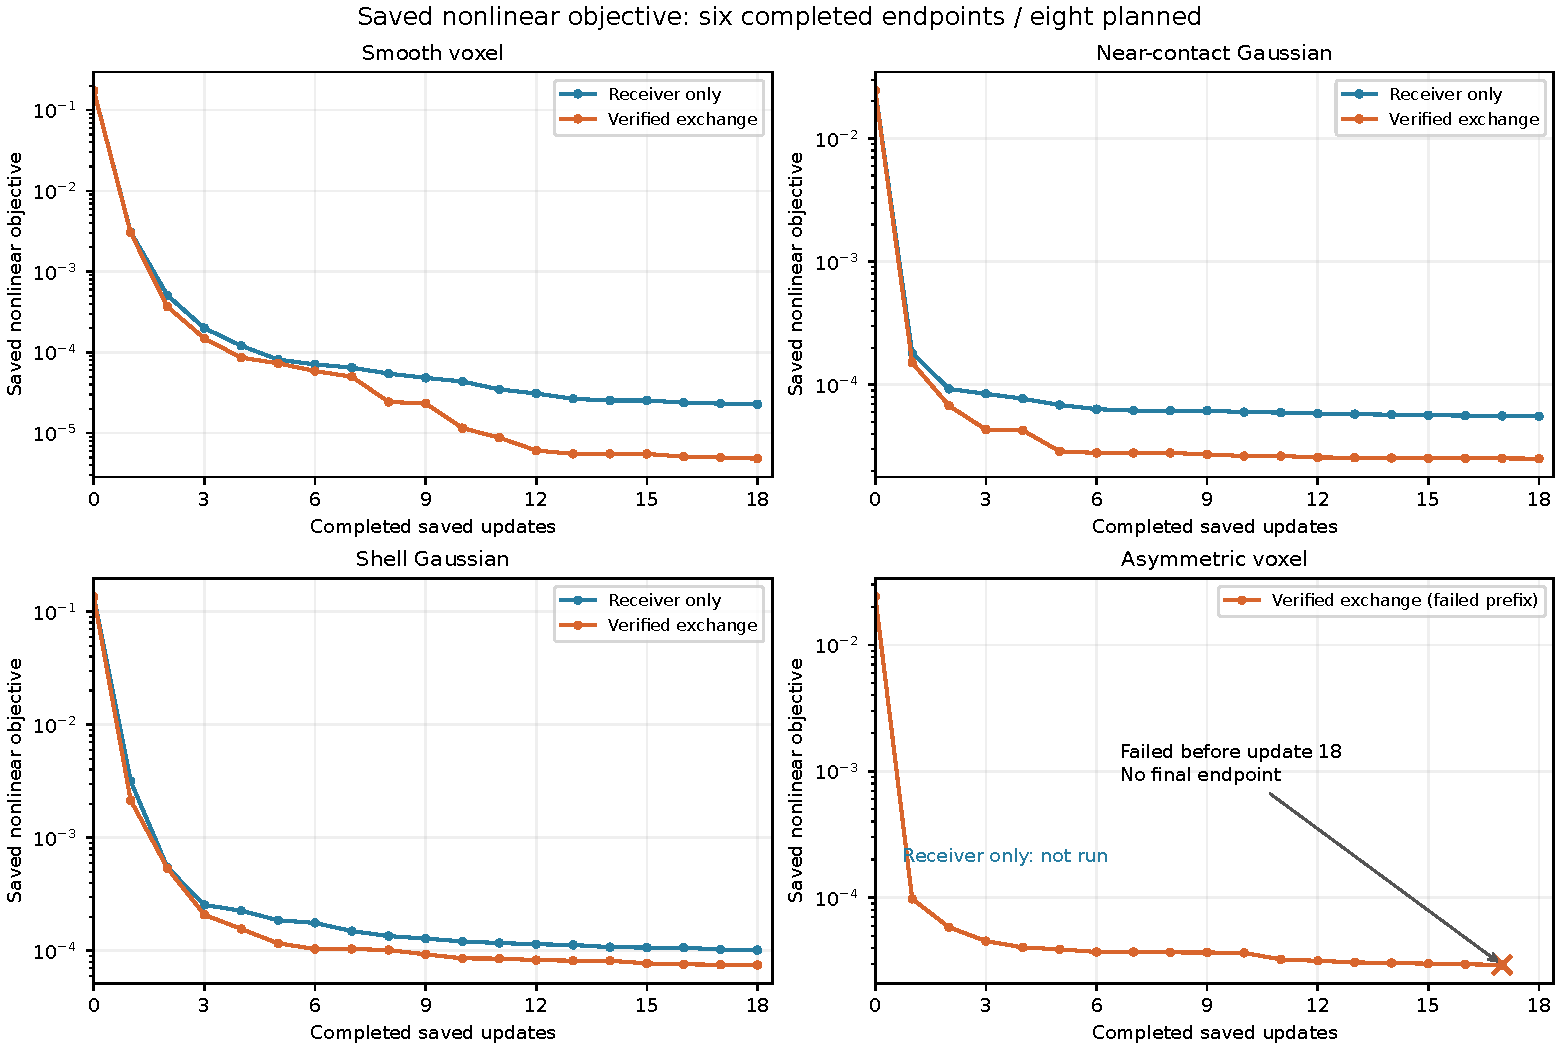
\includegraphics[width=.93\linewidth]{figures/nonlinear_closure_v1/nonlinear_objective_curves.pdf}
\caption{Accepted nonlinear objectives for the three complete pairs and the separate fourth-object prefix. The latter has no completed receiver-only comparator. Its failure and the unrun baseline remain in the eight-job denominator.}
\end{figure}

\section{Offline initial opportunity and bounded paths}
The declared initial domain contains $k(154-k)$ replacements: 600, 1168, and 2208 at $k=4,8,16$. All feasible endpoints are labeled in the 96 available cells. The 2016 late-state prerequisite exclusion leaves three unrun cells in the 99-cell denominator. Teacher labels never enter proposal, ranking, acceptance, or threshold selection.

For each complete object, we sum the positive full-dictionary best gain over its nine initial cells. Dividing the sum of anchor top-one verified/no-op gains by this denominator measures ranking capture. Dividing the sum of best gains achievable within the fixed incoming pool measures candidate coverage. Ranking capture ranges from 0.97302 to 0.99985, with median 0.99538; short-pool coverage ranges from 0.49119 to 0.95307, with median 0.72951. These are weighted one-decision opportunities, not deployed trajectory improvement fractions. The incomplete object is displayed with its observed six-cell scope and is excluded from ten-complete-object summaries.

\begin{figure}[htbp]\centering
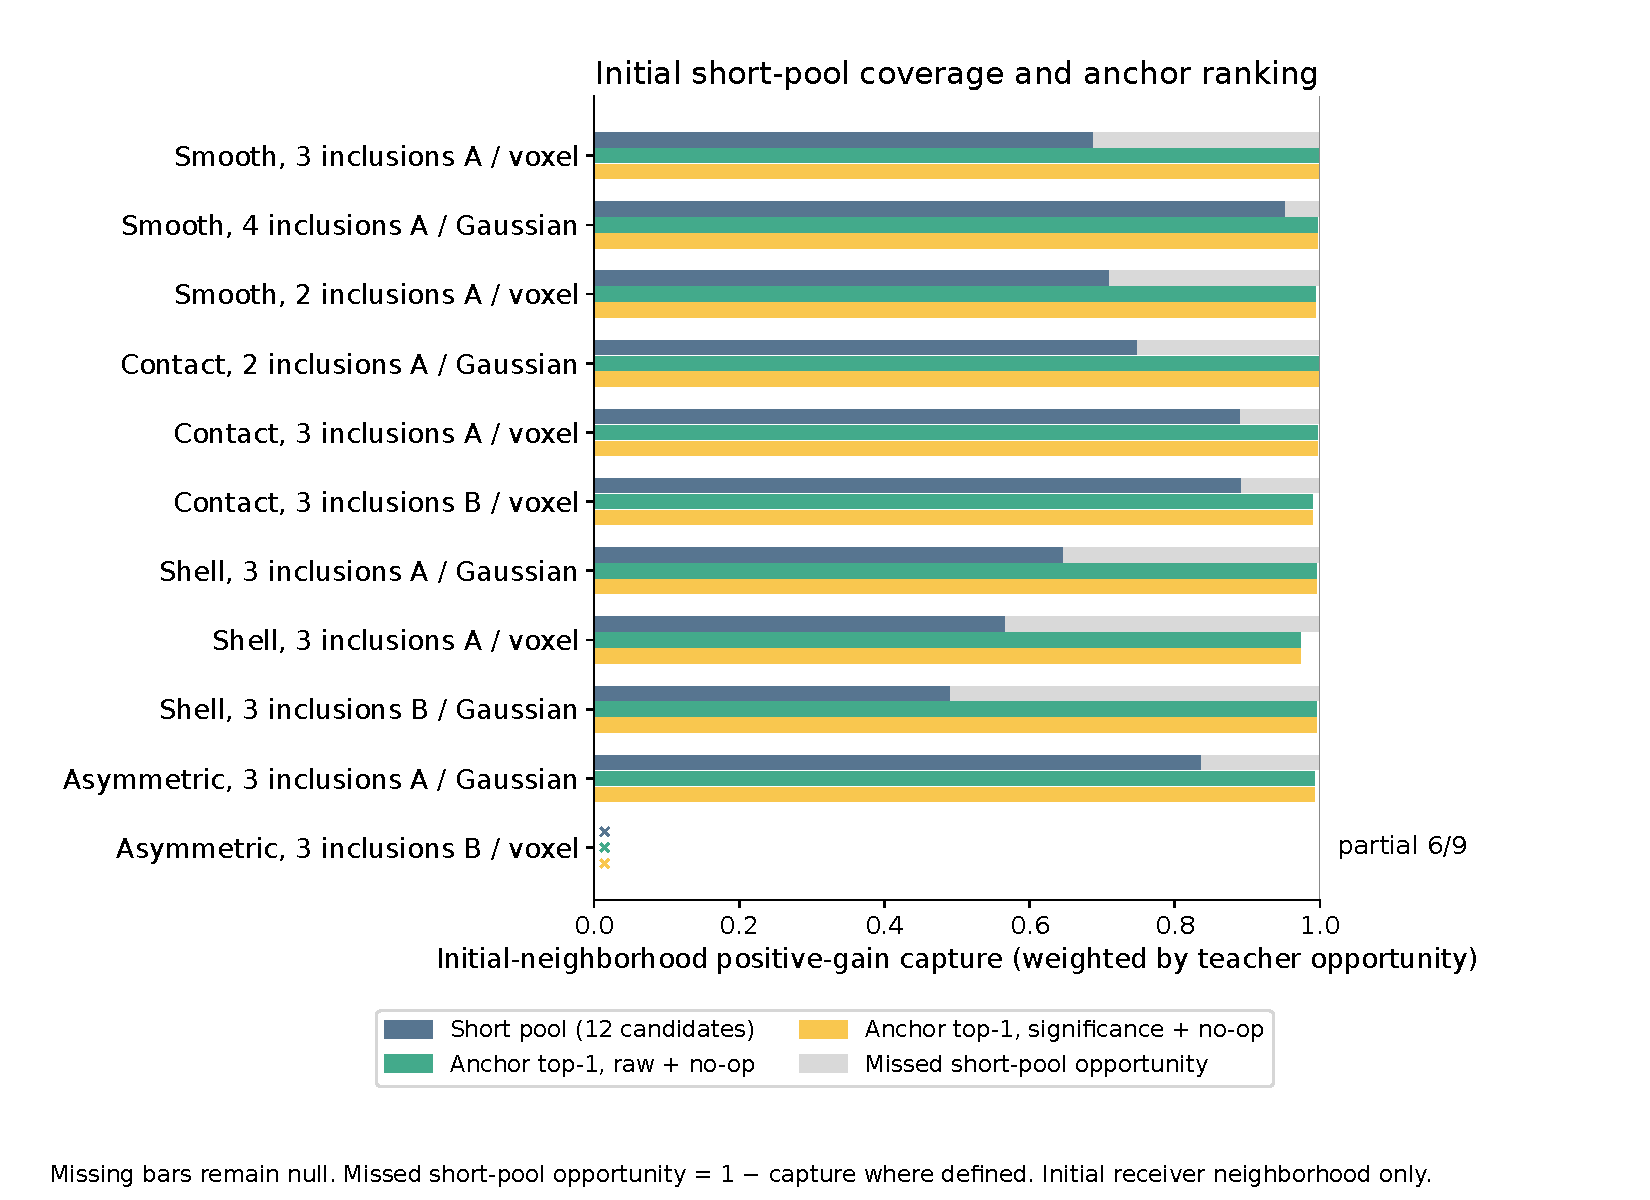
\includegraphics[width=.94\linewidth]{figures/coverage_closure_v2/initial_opportunity.pdf}
\caption{Initial receiver-neighborhood opportunity, separating reduced ranking from acquisition into the frozen 12-atom pool. Missing cells are not imputed.}
\end{figure}
\begin{figure}[htbp]\centering
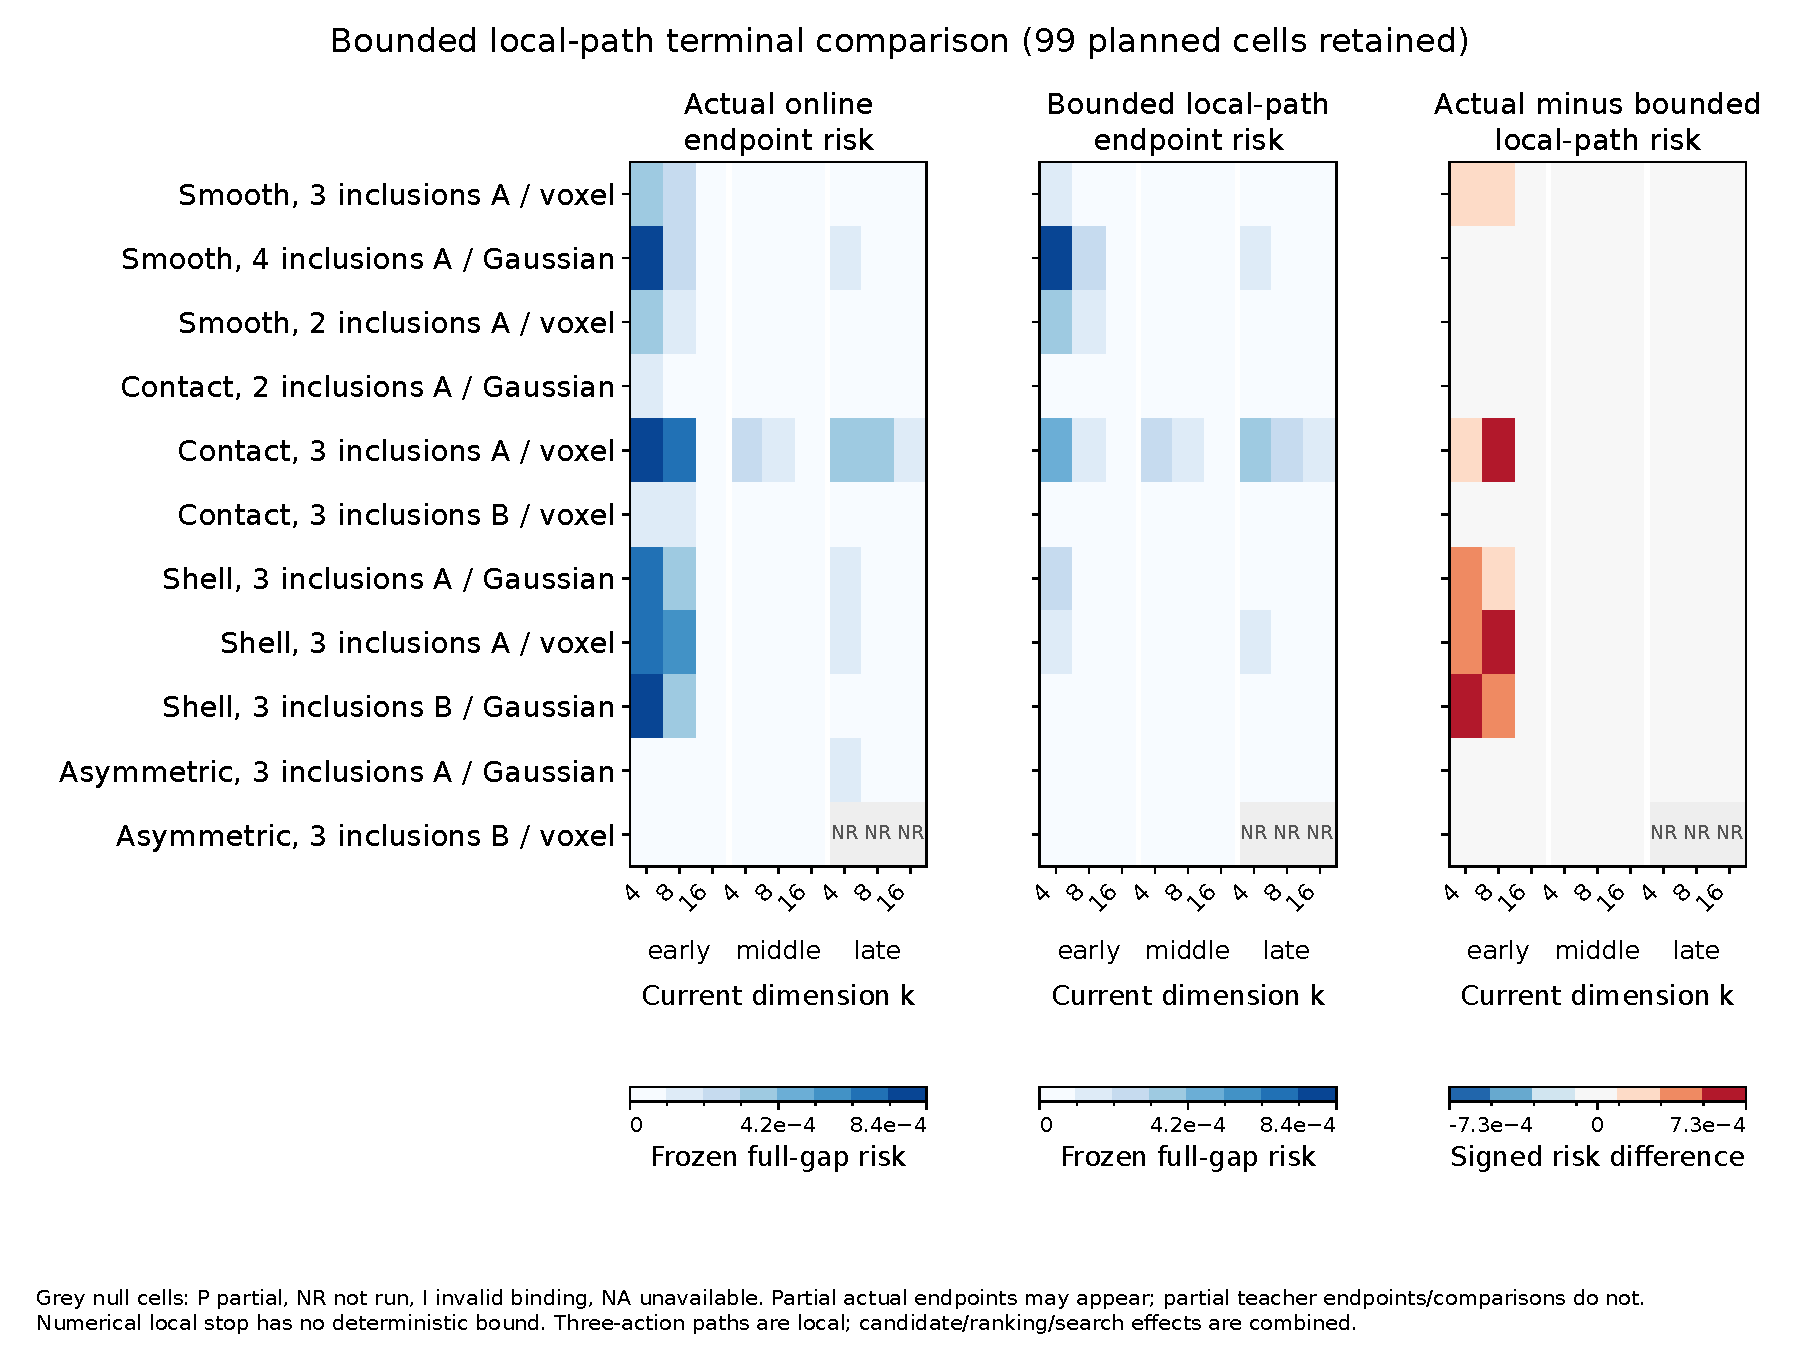
\includegraphics[width=.98\linewidth]{figures/coverage_closure_v2/bounded_path_risk.pdf}
\caption{Online and offline bounded-path final gaps. The teacher recomputes a full local one-swap neighborhood at each accepted step and stops after at most three actions. It is not a global oracle. Five online paths outperform the greedy teacher path, 90 teacher paths outperform deployment, and one differs only within the evaluation floor. These comparisons combine candidate coverage, ranking, and search interactions.}
\end{figure}


\section{Closed costs and physical-action scope}
The authoritative final ledger has 61 closed attempts with matched start/end records, comprising 57 zero and four nonzero exits. All four failed attempts retain their fees. The only additive quantities are historical carry 4889.515~s, closure occupation 15072.343~s and rejected preflight 0.202~s: total 19962.060~s. Successful preflights, child walls and A--I stage walls are already nested inside those occupation intervals.
\begin{table}[htbp]\centering\small
\caption{Mutually exclusive campaign fees. Offline diagnostics are not online deployment work.}\label{tab:closed-cost}
\begin{tabular}{lr}\toprule
Scope&Occupied wall (s)\\\midrule
Historical carry&4889.515\\
Physical threshold replay&268.749\\
Additional frozen objects&1158.673\\
Noisy frozen residuals&895.250\\
Constrained nonlinear transfer&3704.671\\
Offline coverage/path diagnosis&9039.907\\
Gate and failed setup&5.093\\
Rejected preflight outside occupation&0.202\\\midrule
Total&19962.060\\\bottomrule
\end{tabular}\end{table}

Stage views distinguish common physical setup, receiver, anchor, incoming pool, endpoint/score computation, $Jx/Jd$ checks, acceptance/rejection, offline teacher/evaluation and nonlinear work. The full ledger retains missing allocations as null. Cached Gaussian teacher labels pay the dense-$J$ acquisition once; logical cached directions do not add new physical RHS. Voxel teacher directions retain actual block-solve counters. Matrix actions, uploads, SVD, ordinary adjoint and full-adjoint counts remain distinct.

Shared frozen setup was not independently repeated as a cold receiver-only timing. Thus no cold incremental wall is manufactured by allocating a common cache to individual candidates. The three nonlinear pairs independently pay their own setup and are timed once each; their child-wall differences are 363.44, 302.77 and 186.39~s. Rejected finalists and the incomplete fourth trajectory remain charged. The maximum monitored device usage, 2692~MiB, includes other device activity and is not a policy-specific allocated-memory estimate.



\section{Historical controls and independent validation limits}
The original structural material repair exceeds its specified direct current enlargement in 72/72 smooth and 36/36 sharp comparisons. Equal-real-rank material Krylov repair exceeds it in all those comparisons. Paid paired warm starts require 1.416 times matched PCG wall time and increase the recorded full-wave right-hand sides from 66 to 342. These results constrain solver interpretations; they are not overwritten by conditional exchange. TSOM-inspired banks are not native TSOM or FFT-TSOM runs.

Five original normalized closure checks miss tolerance despite absolute $H$ distances $1.06\times10^{-15}$--$3.43\times10^{-14}$ and Schur condition numbers 1.00020--1.00093. Precision traces support cancellation followed by small-denominator amplification, rather than Schur ill-conditioning or proven underflow. All failures remain in the historical archive. Four sharp-target full-model relative material errors are 0.755,0.750,0.560,0.906, limiting claims about interface recovery for that acquisition. The coarse high-contrast sphere has 21.40\% continuum discrepancy.

A separate moderate sphere has 0.252\% aggregate field error and 0.731\% uniform-material derivative error against independent vector Mie at the finest tested grid. This validates that sphere and uniform derivative; it does not independently certify every voxel tangent or every nonradial target. Coarse 12$^3$ inverse states versus 14$^3$ truth generation elsewhere constitute finer-grid checks within the same DDA family.

The broad from-scratch current-ranking study covers 15 observed objects and 258/288 planned budget cells, with failures, missing references and deferred noise retained. Its material-aware finite ranking has median object-summed receiver risk ratio 1.0947; six objects improve. Receiver-centered conditional exchange asks a narrower question and does not overturn that negative result. The common-candidate $2\times2$ diagnostic, rather than the earlier 0.1171 finite/first-order aggregate ratio, isolates finite-displacement curvature cost.

\section{Reproducibility and scope of the evidence package}
The package provides the locked inputs, code and dependency hashes, state and action arrays, completed/failure receipts, analysis and redraw scripts. Actual imported module paths and hashes bind the execution epoch; parser success or a hash without a runtime receipt is not execution evidence. Public Python must preserve executable numerical expressions exactly. Privacy configuration and transport receipts are kept outside the executable research source.

Forty-two hash-identified external/vendor modules remain required for full GPU physics replay. If they cannot be redistributed, the public artifact is an evidence/reanalysis package with external kernel requirements, not a fully self-contained GPU rerun bundle. The local archive retains all versions, monitor failures and measured fees. Complete test and source checks are recorded in the reproducibility report.

The archive file HISTORICAL\_SUPPLEMENT\_ARCHIVE.tex preserves the extended historical derivations and datasets. They support interpretation but are not presented as additional independent validation of the frozen exchange rule.
\begin{thebibliography}{99}
\bibitem{r1} Y. Zhong and X. Chen, ``An FFT Twofold Subspace-Based Optimization Method for Solving Electromagnetic Inverse Scattering Problems,'' \emph{IEEE Trans. Antennas Propag.}, vol. 59, no. 3, pp. 914--927, 2011, doi: 10.1109/TAP.2010.2103027.
\bibitem{r2} X. Ye and X. Chen, ``Subspace-Based Distorted-Born Iterative Method for Solving Inverse Scattering Problems,'' \emph{IEEE Trans. Antennas Propag.}, vol. 65, no. 12, pp. 7224--7232, 2017, doi: 10.1109/TAP.2017.2766658.
\bibitem{r3} X. Chen, \emph{Computational Methods for Electromagnetic Inverse Scattering}. Wiley--IEEE Press, 2018, Secs. 6.3.1 and 6.4.2.
\bibitem{r4} E. de Sturler, S. Gugercin, M. Kilmer, S. Chaturantabut, C. Beattie, and M. O'Connell, ``Nonlinear Parametric Inversion Using Interpolatory Model Reduction,'' \emph{SIAM J. Sci. Comput.}, vol. 37, no. 3, pp. B495--B517, 2015, doi: 10.1137/130946320. Author preprint: arXiv:1311.0922.
\bibitem{r5} M. Kartmann, T. Keil, M. Ohlberger, S. Volkwein, and B. Kaltenbacher, ``Adaptive Reduced Basis Trust Region Methods for Parameter Identification Problems,'' 2024, doi: 10.1007/s44207-024-00002-z. Author full text: arXiv:2309.07627v3.
\bibitem{r6} T. Bui-Thanh, K. Willcox, O. Ghattas, and B. van Bloemen Waanders, ``Goal-Oriented, Model-Constrained Optimization for Reduction of Large-Scale Systems,'' \emph{J. Comput. Phys.}, vol. 224, no. 2, pp. 880--896, 2007, doi: 10.1016/j.jcp.2006.10.026.
\bibitem{r8} A. Gaul, M. H. Gutknecht, J. Liesen, and R. Nabben, ``A Framework for Deflated and Augmented Krylov Subspace Methods,'' \emph{SIAM J. Matrix Anal. Appl.}, vol. 34, no. 2, pp. 495--518, 2013, doi: 10.1137/110820713.
\bibitem{r11} B. T. Draine and P. J. Flatau, ``Discrete-Dipole Approximation for Scattering Calculations,'' \emph{J. Opt. Soc. Am. A}, vol. 11, no. 4, pp. 1491--1499, 1994. Publisher record.
\bibitem{r16} X. Chen, Y. Zhong, and K. Agarwal, ``Subspace Methods for Solving Electromagnetic Inverse Scattering Problems,'' \emph{Methods and Applications of Analysis}, vol. 17, no. 4, pp. 407--432, 2010.
\bibitem{r17} Y. Zhong and X. Chen, ``Twofold Subspace-Based Optimization Method for Solving Inverse Scattering Problems,'' \emph{Inverse Problems}, vol. 25, art. 085003, 2009, doi: 10.1088/0266-5611/25/8/085003.
\bibitem{r18} X.-D. Chen, ``Subspace-Based Optimization Method for Solving Inverse-Scattering Problems,'' \emph{IEEE Trans. Geosci. Remote Sens.}, vol. 48, no. 1, pp. 42--49, 2010, doi: 10.1109/TGRS.2009.2025122.
\bibitem{r19} K. Xu, Y. Zhong, R. Song, X. Chen, and L. Ran, ``Multiplicative-Regularized FFT Twofold Subspace-Based Optimization Method for Inverse Scattering Problems,'' \emph{IEEE Trans. Geosci. Remote Sens.}, vol. 53, no. 2, pp. 841--850, 2015, doi: 10.1109/TGRS.2014.2329032.
\end{thebibliography}

\end{document}
